
\documentclass[10pt, conference, compsocconf]{IEEEtran}

\usepackage{amsmath}
\usepackage{graphics}
\usepackage{subfigure}
\usepackage{graphicx}
\usepackage{algorithm}
%\usepackage{algorithm2e}
\usepackage{algorithmic}


\newtheorem{definition}{Definition}[section]





\begin{document}
%
% paper title
% can use linebreaks \\ within to get better formatting as desired
\title{FPGA Based Efficient Binary Heap Implementation With Hole Minimization}


% author names and affiliations
% use a multiple column layout for up to two different
% affiliations

\author{\IEEEauthorblockN{Monjur Alam and Sushil K. Prasad}
\IEEEauthorblockA{Department of Computer Science\\
Georgia State University\\
Email: malam5@students.gsu.edu, sprasad@gsu.com}
%\and
%\IEEEauthorblockN{Sushil K. Prasad}
%\IEEEauthorblockA{Georgia State University\\
% Email: sprasad@gsu.com}
}

% conference papers do not typically use \thanks and this command
% is locked out in conference mode. If really needed, such as for
% the acknowledgment of grants, issue a \IEEEoverridecommandlockouts
% after \documentclass

% for over three affiliations, or if they all won't fit within the width
% of the page, use this alternative format:
%
%\author{\IEEEauthorblockN{Michael Shell\IEEEauthorrefmark{1},
%Homer Simpson\IEEEauthorrefmark{2},
%James Kirk\IEEEauthorrefmark{3},
%Montgomery Scott\IEEEauthorrefmark{3} and
%Eldon Tyrell\IEEEauthorrefmark{4}}
%\IEEEauthorblockA{\IEEEauthorrefmark{1}School of Electrical and Computer Engineering\\
%Georgia Institute of Technology,
%Atlanta, Georgia 30332--0250\\ Email: see http://www.michaelshell.org/contact.html}
%\IEEEauthorblockA{\IEEEauthorrefmark{2}Twentieth Century Fox, Springfield, USA\\
%Email: homer@thesimpsons.com}
%\IEEEauthorblockA{\IEEEauthorrefmark{3}Starfleet Academy, San Francisco, California 96678-2391\\
%Telephone: (800) 555--1212, Fax: (888) 555--1212}
%\IEEEauthorblockA{\IEEEauthorrefmark{4}Tyrell Inc., 123 Replicant Street, Los Angeles, California 90210--4321}}




% use for special paper notices
%\IEEEspecialpapernotice{(Invited Paper)}




% make the title area
\maketitle


\begin{abstract}
Heap can be used as a priority queue implementation for wild variety of algorithms like routing, anomaly prioritization, etc. It is incumbent to design an efficient parallel operation of priority queue to ensure Quality-of-Service (QoS) guarantees. There are some intrinsic limitation for the realization of truly parallel operation for such algorithm. Some authors provide some parallel solutions \cite{fpga1,fpga2,fpga3}; but they never focus on a serious issue like {\it hole}. All of these approaches incur a lot of hardware cost by producing {\it hole} in the heap. In this paper we propose a hardware realization of parallel binary heap as an application of web based anomaly prioritization. The heap is implemented in pipelined fashion in FPGA platform. The propose design takes $O(1)$ time for all operations by ensuring minimum waiting time between two consecutive operations. We present the various design issues and hardware complexity. We explicitly analyze the design trade-offs of the proposed priority queue implementations.

\end{abstract}

\begin{IEEEkeywords}
Web Anomaly, FPGA, Priority Queue, Verilog;

\end{IEEEkeywords}


\IEEEpeerreviewmaketitle



\section{Introduction}
Network based anomaly detection deals with score calculation and prepares a ranking for all packets based on that score. Due to high network congestion, it is incumbent to provide an efficient interface that can handle prioritization of packets based on the score assigned. As software based application inherently provides slower interface, the hardware based prioritization interface is necessary. Based on the priority, the interface will take some decisions (either pass or drop). For a high speed traffic, it is required to process these tasks in parallel.

Implementation of parallel priority queue will solve this requirement. A priority queue (PQ) is a data structure in which each element has a priority and a dequeue operation removes and returns the highest priority element in the queue. PQs are the most basic component for scheduling, mostly used in routers, event driven simulators \cite{fpga1}, etc. There are several hardware based PQs implementations that  are usually implemented by either ASIC chips \cite{hw1,hw2,hw9} or FPGA \cite{fpga1,fpga2,fpga3}. But, all of them suffer some limitations and not applied to all applications.

In the literature, several hardware-based priority queue architectures have been proposed \cite{hw8,hw9}. All of these
schemes have one or more shortcomings. The {\it Systolic Arrays} and {\it Shift Registers} based approaches \cite{hw8,hw9}, for example, are not scalable and require much hardware, more specifically, it require $O(n)$ comparators for $n$ nodes. FPGA based pipelined heap is presented by Ioannou {\it et. al} \cite{fpga1}. This architecture is very much scalable and can run for 64K nodes without compromising performance. The major drawback of this design is that it takes at least 3 clock cycles to complete a single stage. More over, it never address the {\it hole} generated by parallel {\it delete} operation followed by an {\it insertion}. The calendar queues implemented by \cite{hw1} can only accommodate a small fixed set of priority values since a large priority set would require extensive hard-ware support.

We have implemented a software based anomaly detection mechanism where a score is assigned to each packet. We apply Markov based model for score calculation. A FPGA based parallel binary heap is implemented for score prioritization. We present the various design issues and hardware complexity. The pipeline architecture ensures no waiting time for any operation except the {\it deletion} one which has to wait for a single cycle. Each of {\it insert} and {\it delete} operation takes $O(1)$ time. We also evaluate the design trade-offs of the proposed priority queue implementations. Our design takes care the "hole" created by {\it delete} operation. We minimize the {\it hole} at the time of {\it insertion}.

A Summary of the contents of the sections to follow: Section II contains an overview and the art of literature related to the work. Our proposed design including different design trade-off is presented in section III. Section IV illustrates the implementation result along with the performance comparison with existing designs. Section V concludes the paper and identifies some directions for future research.

\section{Preliminary and Related Work}
\subsection{Web Based Anomaly}

\begin{figure}[h]
\centering
%,height=2.2in
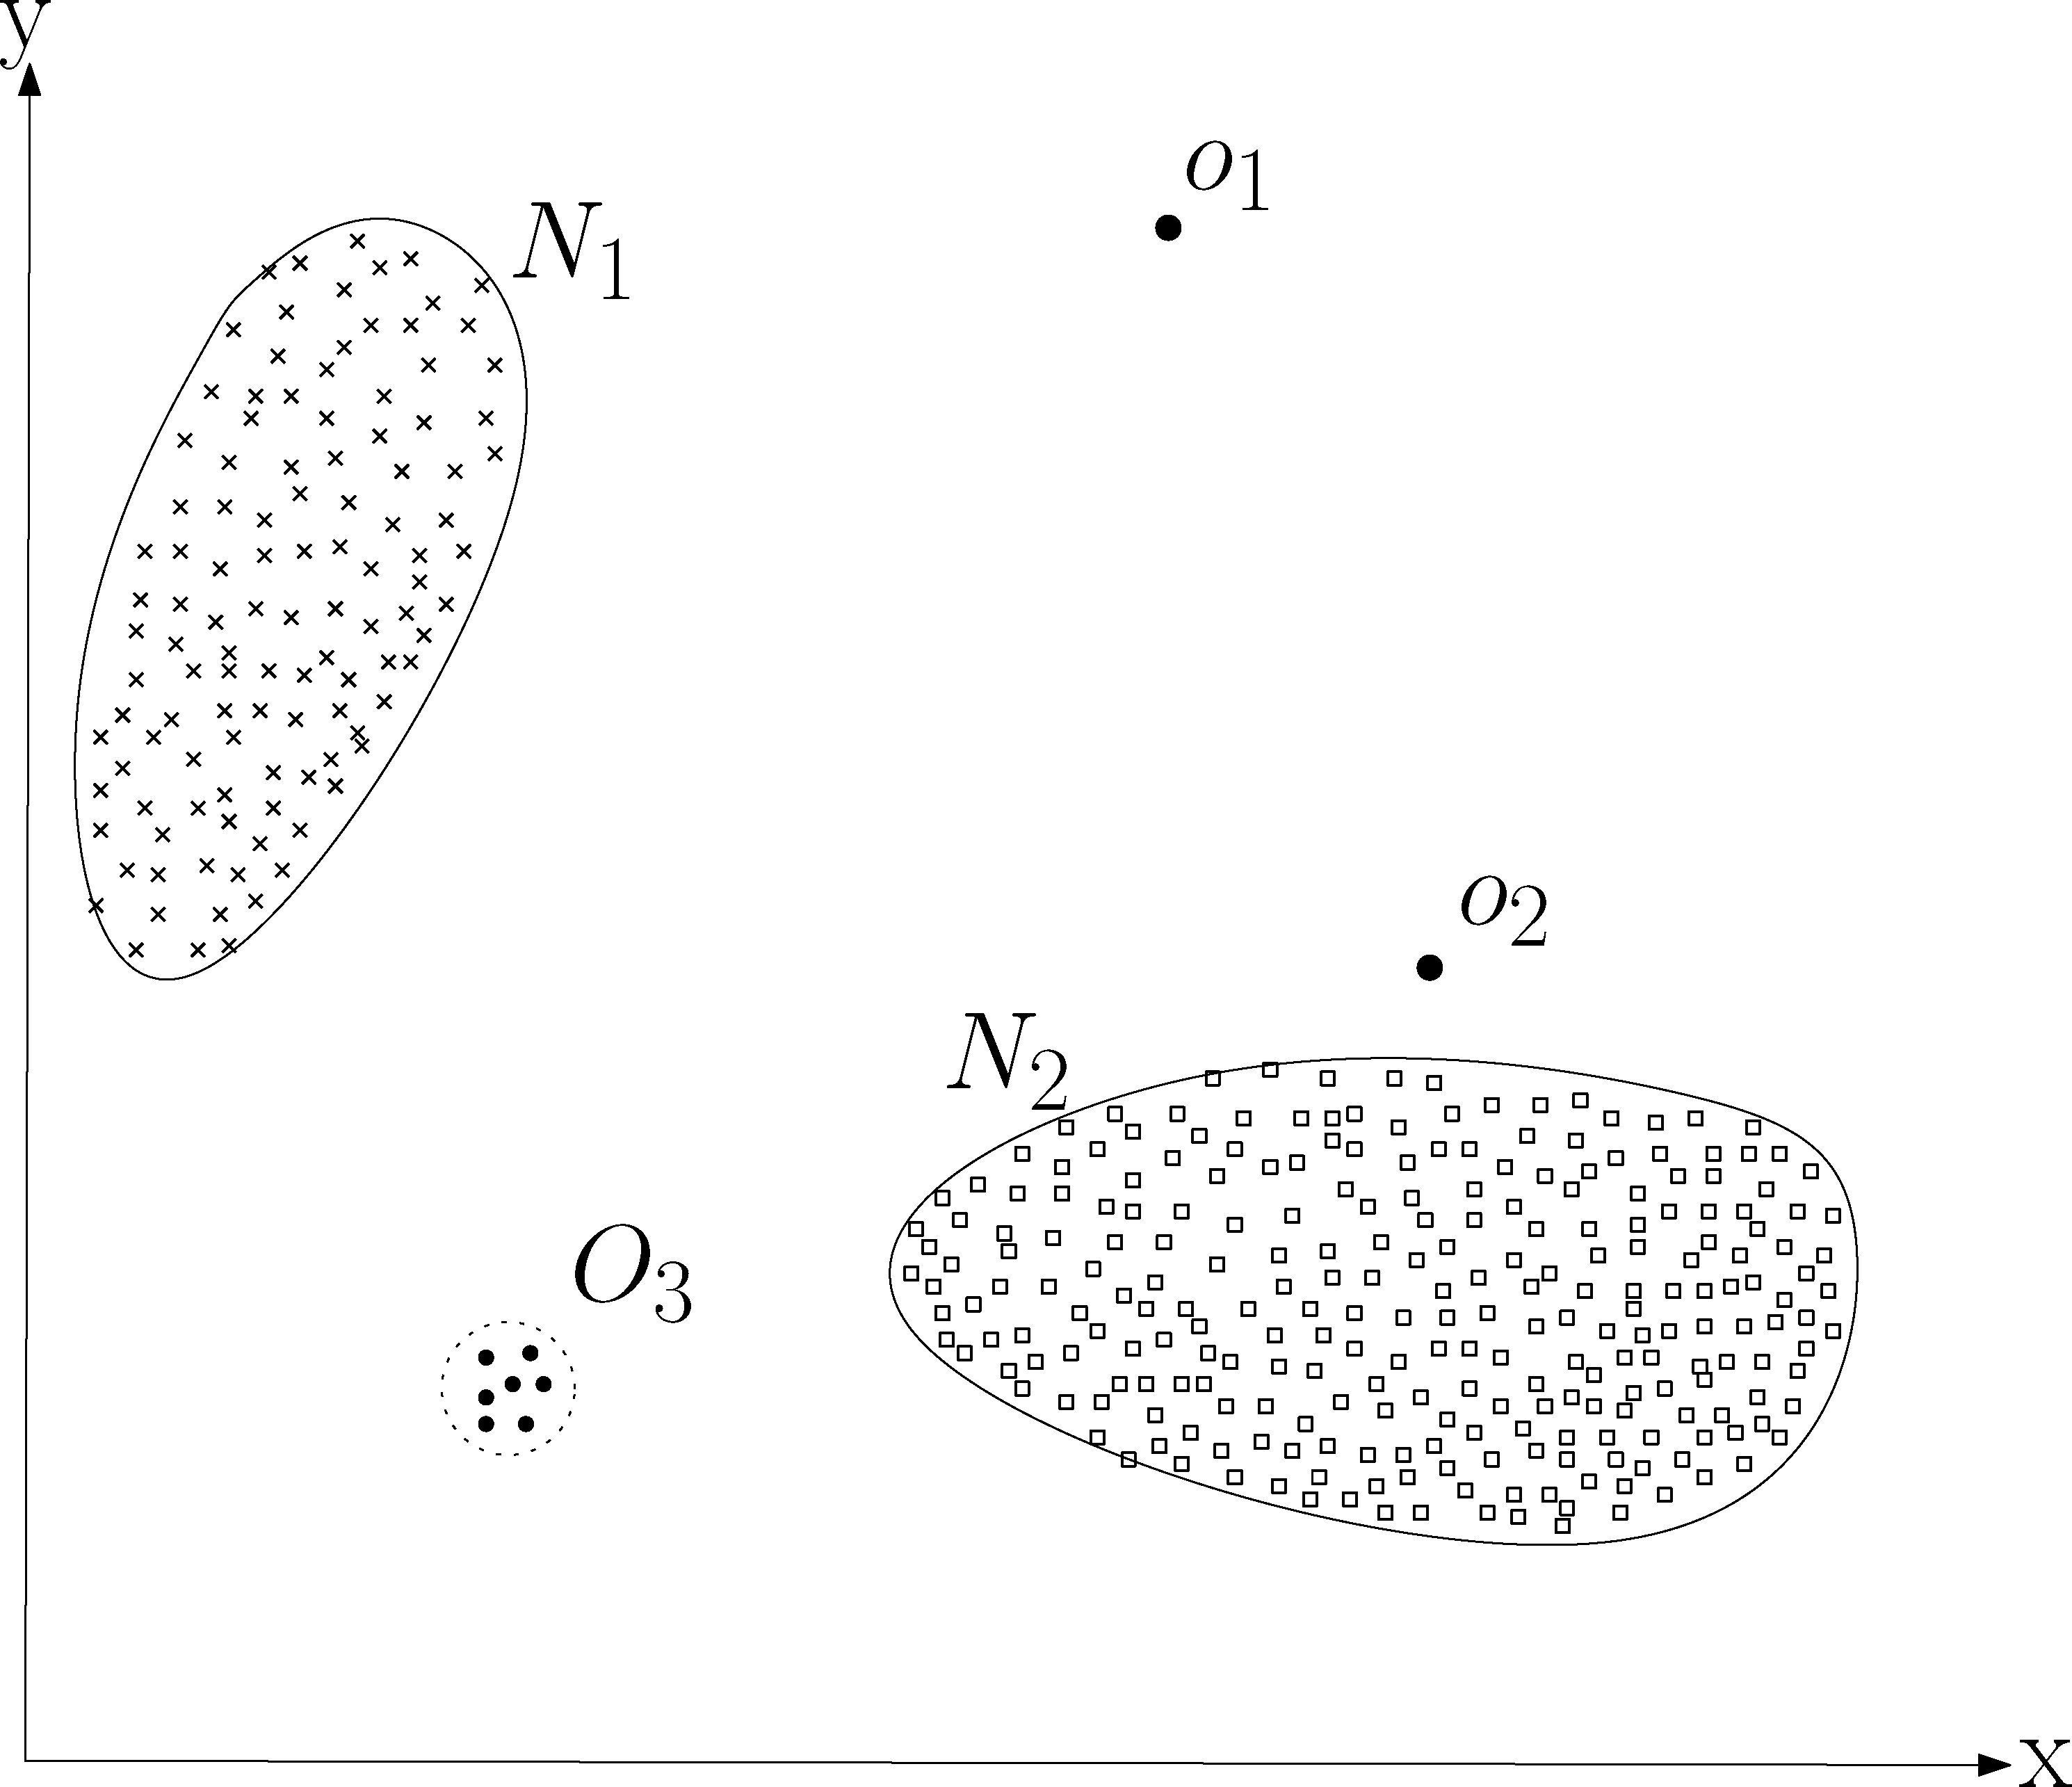
\includegraphics[width=4cm] {Figures/anomaly_fig1}
\caption [Illustrating anomalies in a two-dimensional data set.]{Illustrating anomalies in a two-dimensional data set \cite{1}.}
\label{image1}
\end{figure}

Anomaly detection refers to the problem of finding patterns in data that do not conform to a well defined notion of normal behavior. We often refer these nonconforming patterns as anomalies or outliers. Fig.~\ref{image1} depicts  anomalies in a simple two-dimensional data set \cite{1}. There are two normal regions $N_1$ and $N_2$ for the data since most observations reside in these regions. The points $o_1$ and $o_2$ and all the points in region $O_3$ are considered as anomalies as theses points are sufficiently far away from the two normal regions. We can consider net work packet in each region as data set. Each packet belongs to a particular set based on its score calculation.

\subsubsection{Score Calculation}
\begin{figure}[h]
  \centering
  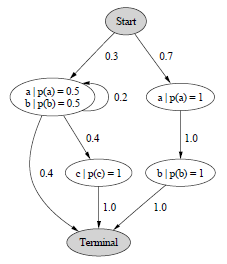
\includegraphics[width=4cm]{Figures/anomaly3.png}
      \caption{Markov Model Example \cite{baum}.}
    \label{anomaly3}
\end{figure}
Among several methods, Markov model is one to calculate score for each packets \cite{baum}. The Markov model (MM) can be viewed as a probabilistic finite state automaton (PFSA) which generates sequences of symbols. The output of the Markov model consists of all paths from its start state to its terminal state. A probability value can be assigned to each output transition and the resultant score is calculated as the summation of all transition probability. For example, consider the non-deterministic finite automata (NFA) in Figure \ref{anomaly3}. To calculate the probability of the word `ab', one has to sum the probabilities of the two possible paths (one that follows the left arrow and one that follows the right one). The start state emits no symbol and has a probability of 1. The result is
\begin{eqnarray}
p(w) &=& (1.0 * 0.3 * 0.5 * 0.2 * 0.5 * 0.4) \nonumber \\
     && + (1.0 * 0.7 * 1.0 * 1.0 * 1.0 * 1.0) \nonumber \\
     && + (1.0 * 0.7 * 1.0 * 1.0 * 1.0 * 1.0) \nonumber \\
     &=& 0.706
\end{eqnarray}


Software based score prioritization of network packets are presented by Kruegel {\it et. al} \cite{web}; where the packets with maximum score gets high priority to be processed next. Each time, the score is calculated "on the fly" and it is compared with other set of precalculated scores. Effectively, there is a processing delay to come up with a decision. Moreover, processing parallel packet is not possible here, as the "on the fly" calculation is highly serialized process.

\subsection{Priority Queue}
A priority queue is an abstract data structure that maintains a collection of elements with the following set of
operations by a minimum priority queue $Q$:
\begin{itemize}
\item {\bf Insert: } A number $n_i$ is inserted into the set of candidate number $N$ in $Q$, provided that the new list maintain the priority queue.

\item {\bf Delete:} Find out the minimum number in $Q$ and delete that number from $Q$. Again, after deletion the property of priority queue should be kept unchanged.
\end{itemize}


\begin{figure}[h]
  \centering
  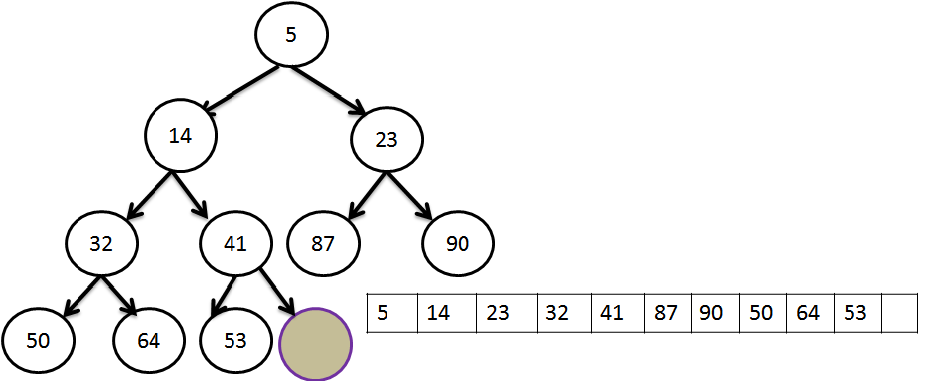
\includegraphics[width=6cm]{Figures/fig2.png}
      \caption{Binary min heap with its array representation.}
    \label{fig2}
\end{figure}

\subsubsection{Priority Queue Implementation}
Priority queue can be implemented by using binary heap data structure.
\begin{definition}
A min-heap is a binary tree $H$ such that (i) the data contained in each node is less than (or equal to) the data in that node’s children and (ii) the binary tree is complete.
\end{definition}

Figure \ref{fig2} shows the binary min heap ($H$). The root of $H$ is $H[1]$, and given the index $i$ of any node in $H$, the indices of its parent and children can be determined in the following way:
\begin{eqnarray*}
parent[i] &=&  \lfloor i/2 \rfloor \\
leftChild[i] &=& 2i\\
rightChild[i] &=& 2i + 1
\end{eqnarray*}

The insertion algorithm on the binary min heap $H$ is as follow:
\begin{itemize}
\item Place the new element in the next available position (say $i$) in the $H$.
\item Compare the new element $H[i]$ with its parent $H\lfloor i/2 \rfloor$. If $H[i]$ $<$ $H\lfloor i/2 \rfloor$, then swap it with its parent.
\item Continue this process until either (i) the new element’s parent is smaller than or
equal to the new element, or (ii) the new element reaches the root ($H[1]$).
\end{itemize}

\begin{figure}[h]
  \centering
  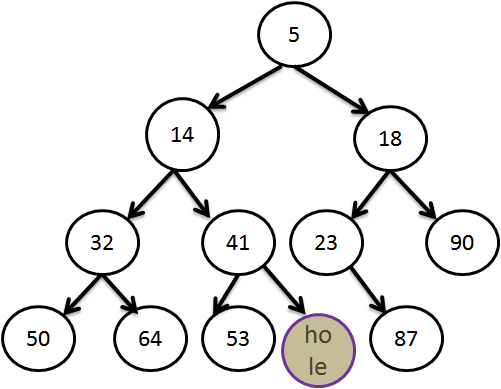
\includegraphics[width=4cm]{Figures/fig3.png}
      \caption{New heap structure after insertion 18.}
    \label{fig3}
\end{figure}

\begin{figure}[h]
  \centering
  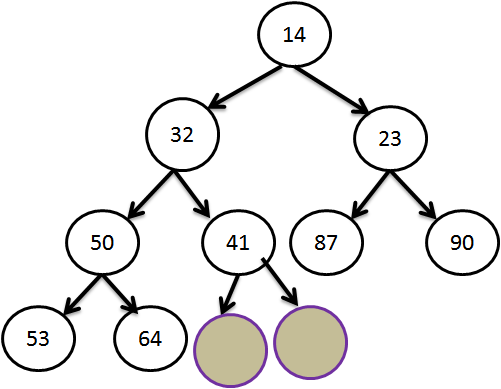
\includegraphics[width=4cm]{Figures/fig4.png}
      \caption{New heap structure after single deletion operation from the original heap shown at figure \ref{fig2}.}
    \label{fig4}
\end{figure}

Figure \ref{fig3} shows the new heap structure after insertion of 18 at the heap presented in Figure \ref{fig2}.

The deletion algorithm is as follow:
\begin{itemize}
\item Return the root $H[1]$ element.
\item Replace the root $H[1]$ by the last element at the last level (say $H[i]$).
\item Compare root with its children and replace the root by its min child.
\item Continue this replacement for each level by comparing $H[i]$ with $H[2i]$ and $H[2i+1]$, un till the parent become less than its children or it reaches to the leaf node.
\end{itemize}

Figure \ref{fig4} depicts the heap structure of single deletion operation from the original heap shown at Figure \ref{fig2}. We can see that 5 was the root element at Figure \ref{fig2}. The updated Figure \ref{fig4} depicts that the 5 is no anymore after the {\it deletion}. Moreover, heap is re-structured according to the {\it deletion} algorithm presented above.


\subsection{Related Work}
Many web anomaly detection techniques have been proposed which applied a set of training data to define a model of normal behaviour. It labelled any data as abnormal that is not included in this model \cite{35,62,160,198,Chr,Fre,Kon}. Several variants of the basic technique have been proposed for network intrusion detection, and for anomaly detection in text data \cite{Moh,Meh,gio}. These approaches assume independence between the different attributes. Some approaches have been introduced that assume the conditional dependencies between the different attributes applying more complex Bayesian networks \cite{Janakiram,Das,Wil}. Rule-based anomaly detection techniques distinguish normal behavior of data instances from anomalies by learning rules. A test instance is termed as anomaly if it is not covered by any such rule. There are two steps for rule-based anomaly detection approach. First, rules are learned from the training data using a rule learning algorithm. A confidence value is associated with every rule. The second step is to search the rule that best captures the test data instance. The anomaly score of the test instance is calculated as the inverse of the confidence associated with the best rule. For example, a typical rule-based system is an expert system where the rules are generated by humans \cite {1,68,111}.

All of the approaches mentioned suffer from two basic problems:
\begin{enumerate}
\item There is no efficient implementation to deal with huge network congestion.
\item prioritization of network traffics are net maintain.
\end{enumerate}

\subsubsection{Anomaly Detection by Using Hardware}
To resolve the first class of difficulty several authors \cite{ah1,ah3} come up with hardware based solution. The intention is to provide very fast interface to process network data. To achieve this goal, Das {\it et. al.} \cite{ah1,ah2} comes up with hardware based solution for anomaly detection. The work comprises of a new Feature Extraction Module (FEM) which summarizes the network behavior. It also incorporates an anomaly detection mechanism using Principal Component Analysis (PCA) as the outlier detection method. The authors of \cite{ah3} propose an FPGA-based reconfigurable architecture for feature extraction of large high-speed networks.

\subsubsection{Parallel Priority Queue}
Several authors have theoretically proved that parallel heap as an efficient data structure to implement priority queue. Prasad {\it et. al.} \cite{pq0,pq3} theoretically illustrate this data structure to show $O(p)$ operations are required with $O(log / n)$ time for $p \leq n$, where $n$ is the number of nodes and $p$ is the number of processor used. The idea is designed for EREW PRAM shared memory model of computation. The many core architecture by \cite{pq2} in GPGPU platform provides multi-fold speed up. Another theoretical approach \cite{pq4} deploys pipeline or tree of processors ($O(log / n$, where $n$ is the number of node) to produce optimize result. The implementation of this algorithm \cite{pq5} is expensive in case of multi-core based architectures

\subsubsection{Hardware Based Priority Queue}
There have been a good number of hardware based priority queue implementations described in the literature \cite{hw1,hw2,hw3,hw5,hw6,hw7,hw8,hw9}.  Pipelined based ASIC implementations can reach $O(1)$ execution time \cite{hw5,hw6}. Due to several limitations, most of the ASIC implementations assist a limited number of nodes and are not scalable for high rate. In \cite{hw7}, a more efficient pipelined heap construction is presented; however their result is a complex hardware implementation requiring many hardware processors or special elements and is very specific to pipelined heaps of particular size. Other hardware implementations are {\it Systolic Arrays} and {\it Shift Registers} \cite{hw8,hw9}. They are both based on an array of $O(n)$ comparators. The responsibility of comparators used here to compare nodes in different level with $O(1)$ step complexity. For the shift register \cite{hw9} based implementations, new inputs are broadcasted to all levels. It requires a global communicator hardware which can connect with all level. The implementation based on {\it Systolic Arrays} \cite{hw8} needs a bigger storage buffer to hold pre-processed data. These approaches are not scalable and require much hardware, more specifically, it require $O(n)$ comparators for $n$ nodes. To overcome the hardware complexity, a recursive processor is implemented by \cite{hw10}; where a drastic hardware is reduced by compromising execution timing cost. Bhagwan and Lin \cite{hw2} designed a physical heap such a way that commands can be pipeline between different levels of heap. The authors in the paper \cite{hw1} give some pragmatic solution of so called {\it fanout} problem mentioned in \cite{hw3}.

For the FPGA based priority queue implementation,  Kuacharoen {\it et. al} \cite{fpga3} implemented the logic presented in \cite{hw3} by incorporating some extra features to ensure the design to be acted as a Real-Time Operating System task scheduler. The major limitation of this paper is that it deals with very few priority levels and a small number of items in the queue at any given time. A hybrid priority queue is implemented by \cite{fpga2} and it ensures high scalability and high throughput. FPGA based pipelined heap is presented by Ioannou {\it et. al} \cite{fpga1}. This architecture is very much scalable and can run for 64K nodes without compromising performance. The major drawback of this design is that it takes at least 3 clock cycles to complete a single stage. More over, it never address the {\it hole} generated by parallel {\it delete} operation followed by an {\it insertion}.

\section{FPGA Based Parallel Heap Implementation}
Like an array representation, heap can be represented by hardware register or FPGA latch. Each level of the heap can be virtually represented by each latch. The size of the latch at each level can be represented as $2^{\beta-1}$, where $\beta$ is the level assuming that root is the level 1. Figure \ref{fig5} shows the different latches do represent the different levels. Here, root node can be stored by $L_1$, the next level with two elements can be stored in $L_2$ and the last level with 3 elements can be stored in $L_4$, although the last level can have max 8 elements.

\begin{figure}[h]
  \centering
  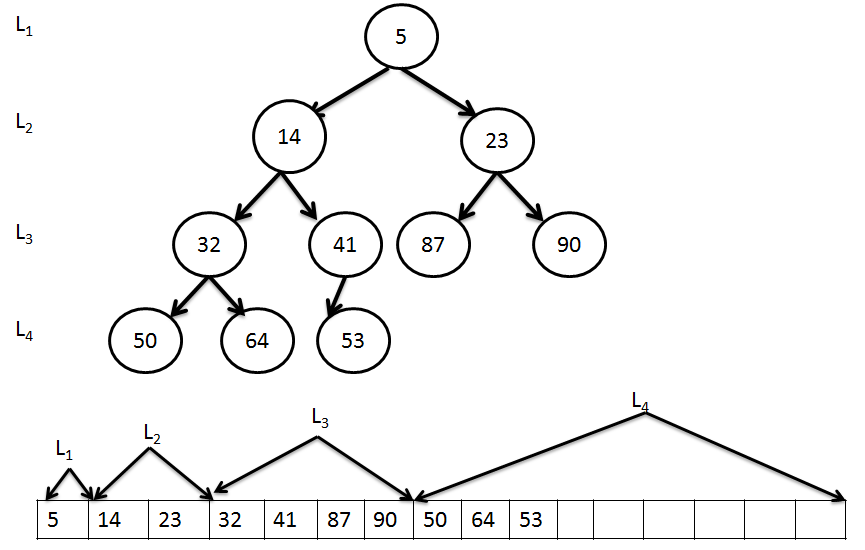
\includegraphics[width=8cm]{Figures/5.png}
      \caption{Storage in FPGA of deferent nodes in binary heap}
    \label{fig5}
\end{figure}

\subsection{Insert Operation}
\begin{figure}[h]
  \centering
  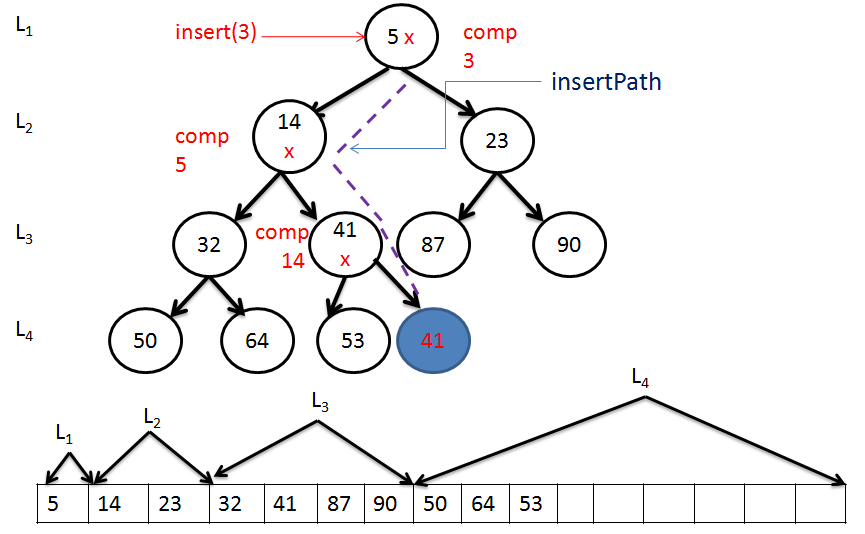
\includegraphics[width=8cm]{Figures/6.png}
      \caption{Insertion path}
    \label{fig6}
\end{figure}

\begin{figure}[h]
  \centering
  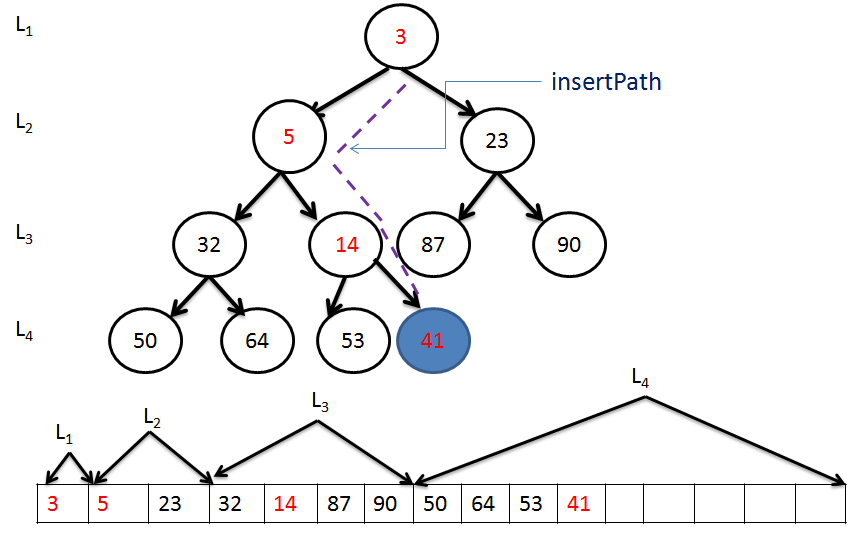
\includegraphics[width=8cm]{Figures/7.png}
      \caption{Contain of latch ($L$) after insertion completed}
    \label{fig7}
\end{figure}

We have already discuss the insert operation which is intimated from the last available node of the heap. This bottom up approach restrict the other operations like delete, replace, etc. to perform in parallel. As deletion means the least element to be deleted and the least element always resides at root in case of min heap; deletion operation should wait till the root is updated by the insert operation. If we insert element 3 in the heap mentioned at Figure \ref{fig5}, followed by delete one element from heap then what will happen? Let us assume nodes at each level get updated by a single clock cycles. That means, in worst case, total 4 clock cycles are required to complete the insert operation in this situation. So, delete operation either has to wait for 4 clock cycles or it will wrongly delete the root, which is 5. So, it is incumbent to insert from root and go down. But, we need to know the path for the new inserted element, otherwise the tree will not be complete binary tree. We have adopted a nice algorithm presented by Vipin {\it et. al} \cite{pq6} in our design. The algorithm is as follow:

\begin{itemize}
\item Let $k$ is the last available node at where new element to be inserted. Let $j$ be the first node of the last level. Then binary representation of $k-j$ will give you the path.
\item Let $k-j = B$, which binary representation is $b_{\beta-1}b_{\beta-2} \cdots b_2b_1$. Starting from root, scan each bit of $B$ starting from $b_{\beta-1}$;
    \begin{itemize}
    \item if $b_i == 0$ ($i \in \{\beta-1,\beta-2, \cdots, 2,1$), then go to left
    \item else go right
    \end{itemize}
\end{itemize}

The Figure \ref{fig6} shows the insertion path for $new$ element to be inserted. For the new element insertion, node at 11 should be filled up. The first node of the last level is at index 8. So, 11-8 = 3, which can be represented as 011. So, starting from root, the path should be $root \rightarrow left \rightarrow right \rightarrow right$ and this can be demonstrated by the Figure \ref{fig6}. After the insertion completion, the contain of the nodes along with the value of latch is presented by the Figure \ref{fig7}.


\subsection{Delete Operation}

There is one conventional approach to delete element from heap. As root resides the min element, deletion always happen from root and the last element is replaced to root. There are two difficulties here:
\begin{enumerate}
\item For sequential operation, it works perfectly file. For, parallel execution of insert/del, $hole$ can be created here. The situation happen after any $insert$ followed by $delete$ operation.
\begin{figure}[h]
  \centering
  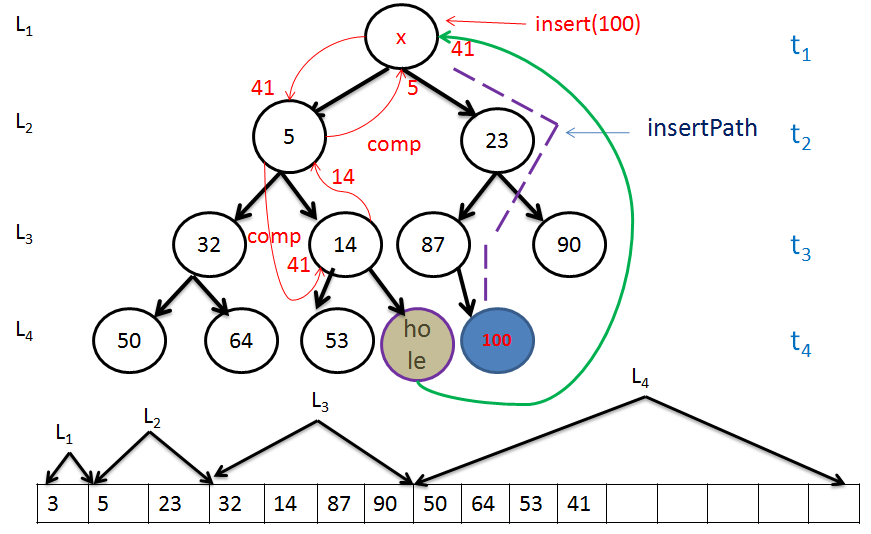
\includegraphics[width=8cm]{Figures/8.png}
      \caption{Hole is the resultant for parallel operation of insert-delete}
    \label{fig8}
\end{figure}

\begin{figure}[h]
  \centering
  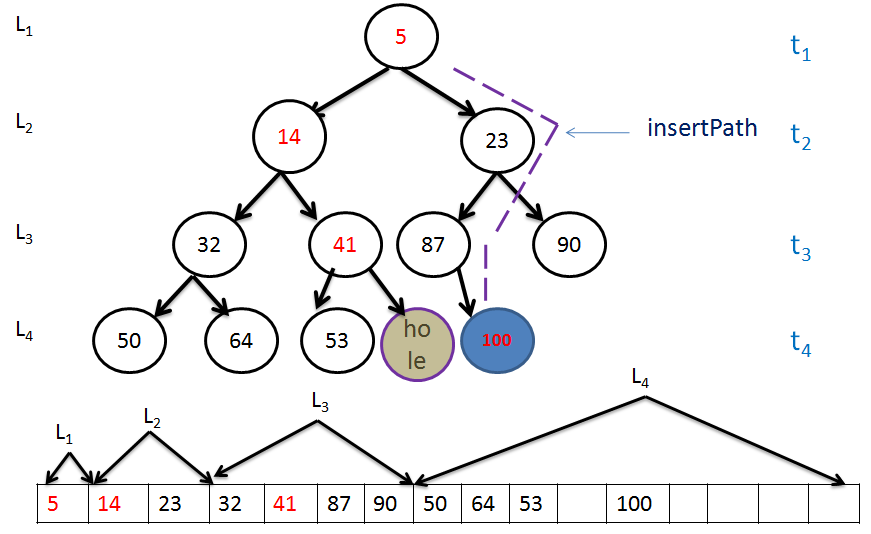
\includegraphics[width=8cm]{Figures/9.png}
      \caption{Contain of latch ($L$) after parallel operation of insert-delete}
    \label{fig9}
\end{figure}

\begin{figure*}[!ht]
  \centering
  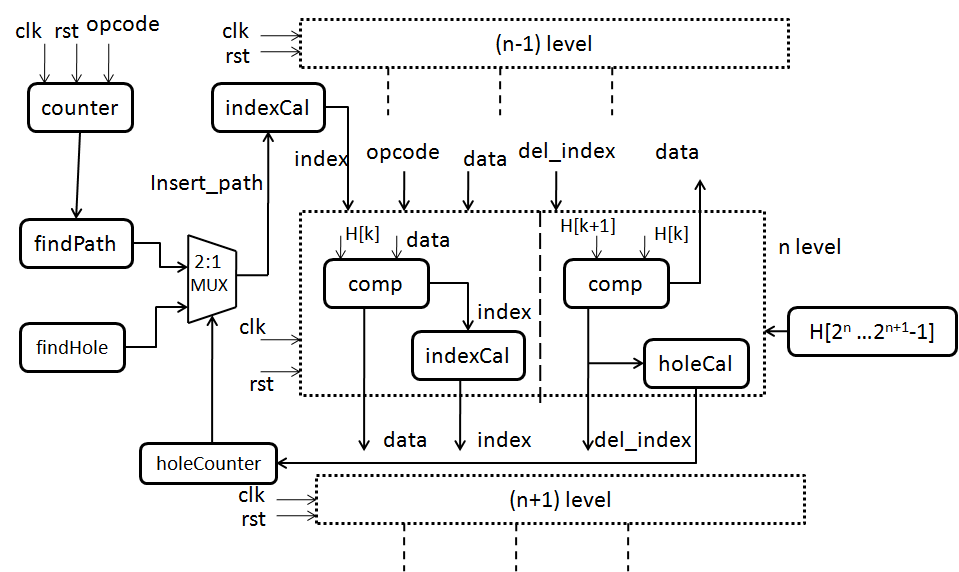
\includegraphics[width=12cm]{Figures/2.png}
      \caption{Top Level Architecture of insert-delete}
    \label{fig2}
\end{figure*}

From the Figure \ref{fig8} we can illustrate this scenario clearly. Let at $t_1$, the operation insert with element 100 is encountered and it is denoted by $insert(100)$. Obviously, the element will be inserted at the last node of last level which is 12. Let, after one clock cycle of $insert$, $delete$ is encountered (say at $t_2$). At, that time, $insert$ was modifying at $L_2$. So, due to $delete$, hole will be created at node 10th as shown in Figure \ref{fig8}. Eventually, when $insert(100)$ will finish, the element 100 will occupy at the position of $H[12]$, but, $H[11]$ will become empty. This situation is illustrated by Figure \ref{fig9}.

Let us assume that $insert$ instruction comes at time $t_i$ and $delete$ instruction comes at $t_j$, where $i, j = 1,2,3, \cdots$ and $j>i$.  Let, operation of either $insert$ or $delete$ takes one clock cycle at any level to complete tasks at that level. It is obvious that, only single node gets modified (if any) for all levels. In general, for any $insert-delete$ combination, $hole$ will be created if $(t_j - t_i) < \beta$, where $\beta$ is the depth of heap.

\item While you replace root by last element of heap, it requires extra clock cycle. Moreover, we need to compare three elements, root and its two children or any node and its children. For hardware perspective, it is cost efficient to compare two elements rather than to compare three elements. More over, it incurs the path delay longer.

\end{enumerate}

So, we should intentionally avoid the root replacement by last element. Let us delete root first and keep it as it is. Fill the root with its least child and follow the algorithm. In this case, we can save one cycle and hardware cost, more specifically, can minimize the path delay. Now, our aim is to minimize {\it hole} by adding logic.

\subsection{Insert-Deletion Logic Implementation}

Figure \ref{fig2} illustrates the top level architecture of {\it insertion-delete} operation. The {\it counter} is used to maintain the total number of element present in the heap. It is incremented by one for {\it insert} operation and decremented by one for {\it deletion operation}. The {\it indexCal} block is used to find the insertion path. We have modified the existing path finding algorithm by \cite{pq6}. We first consider the {\it holeReg} to obtain insertion path. The {\it holeReg} contains the {\it holes} created at {\it deletion} operation. We maintain a {\it holeCounter} to identify a valid {\it hole}. Based on the {\it index}, the heap node is accessed and the node is compared with the present data. Based on the comparison, either the node is updated by present data and the node is passed to the next level as present data, or the node become unchanged and the present data is passed to the next level.

{\bf Deletion :} We maintain {\it del\_index} to find the last deleted node. For example, initially, {\it del\_index} becomes 1 which means root is deleted. The comparator finds the min element between $H[del\_index*2]$ and $H[del\_index*2 + 1]$ and that min gets replace to $H[del\_index]$. Now, {\it del\_index} gets modified with the index of min element. Again the comparator finds the min of the ancestors of the new index and replace the node of new index with that of min one. Each time {\it holeCal} finds if there is a valid child for {\it del\_index}. If there is no valid child, then {\it holeCounter} is incremented by 1 and {\it holeReg} is updated with {\it del\_index}. By this way, we maintain {\it hole}.

\begin{figure*}[!ht]
  \centering
  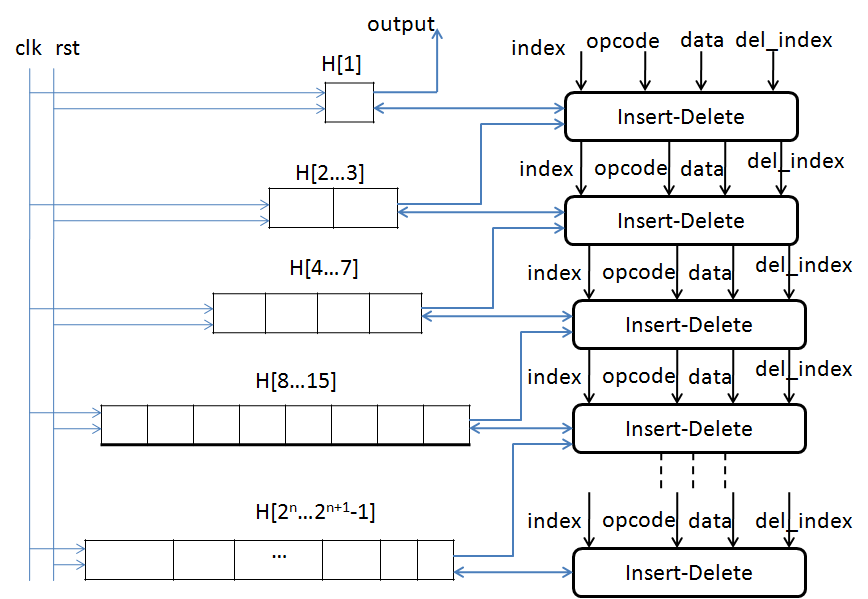
\includegraphics[width=9cm]{Figures/1.png}
      \caption{Pipeline Design Overview}
    \label{fig1}
\end{figure*}


\begin{algorithm}
\label{algo1}
        \caption{Algorithm for $Insert-Delete (data, opcode)$}
\label{algo1}
        \begin{algorithmic}[1]
           % \Procedure{Insert}{data,opcode} %\Comment{The g.c.d. of a and b}
          \IF{(opcode == 1)} %\rcomment{Insertion}
            \STATE{ counter = counter +1;
            }
            \IF{($holeCounter > 0$)}
                \STATE{insert\_path = $findPath(counter, \ holeCounter)$}
            \ENDIF
            \FOR{(0 \TO number of level) }
                \STATE{$index$ = $indexCal(insert\_path)$}
                \IF{($data < H[index]$}
                    \STATE{ $H[index] = data$\\
                    $data = H[index]$
                    }
                \ELSE
                    \STATE{$data = data$ }
                \ENDIF
            \ENDFOR
          \ELSE
          \STATE {
          Remove $H[1]$ \\
          }
          \WHILE{($leftChild[del\_index] \neq NULL \& rightChild[del\_index] \neq NULL$)}
            \IF{($leftChild[del\_index] < rightChild[del\_index]$)}
                \STATE{$H[del\_index] = leftChild[del\_index]$\\
                $del\_index = del\_index *2$
                }
            \ELSE
                \STATE{$H[del\_index] = rightChild[del\_index]$\\
                $del\_index = del\_index *2 + 1$
                }

            \ENDIF

          \ENDWHILE
          \STATE{ $hole\_counter = hole\_counter + 1$\\
          $hole\_reg[hole\_counter] = del\_index$
          }
        \ENDIF

        \end{algorithmic}
\end{algorithm}

The {\it insert-delete} parallel algorithm is presented at Algorithm \ref{algo1}. We use 2:1 multiplexer to select the path based on the value of {\it holeCount}. The logic for {\it findPath} is illustrated at Algorithm \ref{algo2}. The {\it indexCal} block is implemented based on the value of {\it findPath} and the logic is illustrated at Algorithm \ref{algo5}. To calculate the first node of last level is noting but the mathematical expression of $log(\beta)$ where $\beta$ is the level of heap. There is some difficulty to realize this expression in hardware. We express this logic by Algorithm \ref{algo3}.

\begin{algorithm}
\caption{Algorithm for $findPath$(counter, holeCounter)}
\label{algo2}
\begin{algorithmic}[1]
    \IF{($holeCounter > 0$)}
        \STATE{\RETURN $findHole(holeCounter)$\\
        }
    \ELSE
        \STATE{$leaf\_node$ = $findNode(counter)$ \\
        \RETURN ($counter - heap\_level$
        }
    \ENDIF
\end{algorithmic}
\end{algorithm}

\begin{algorithm}
\caption{Algorithm for $findNode(counter)$}
\label{algo3}
\begin{algorithmic}[1]
    \FOR{($i$ = 0;  $2^i < counter$; i = i+1) }
        \STATE{$leaf\_node$ = i+1}
    \ENDFOR
    \RETURN $leaf\_node$
\end{algorithmic}
\end{algorithm}


\begin{algorithm}
\caption{Algorithm for $findHole(hole\_counter)$}
\label{algo4}
\begin{algorithmic}[1]
    \RETURN $holeReg[holeCounter]$
\end{algorithmic}
\end{algorithm}

\begin{algorithm}
\caption{Algorithm for $indexCal(insert\_path)$}
\label{algo5}
\begin{algorithmic}[1]
    \FOR{($i$ = 0 \TO $insert\_path$ bits) }
        \IF{(bit == 0)}
            \STATE{$index_i$ = 2*$index_(i-1)$}
        \ELSE
            \STATE{$index_i$ = 2*$index_(i-1) + 1$}
        \ENDIF
    \ENDFOR
\end{algorithmic}
\end{algorithm}

We have used global clock(clk) and global reset(rst) signal for the each logic block except the combinational logic parts. The clk and rst signals are not mentioned at each figure due to place limitation. The function of {\it findHole} is basically an implementation of stack register and its return value is presented at Algorithm \ref{algo4}.



\subsubsection{Pipeline Design}


To achieve high throughput we need to start one operation before completing the previous operation. So, many operation can be in progress in the tree. To achieve so, we consider our design to take a single clock cycle to perform each stage. For any stage, only one operation ({\it insert, delete}) can be execute at ant time $t$. That is why we need all operation should be started from the top (root) of the tree and proceed towards the bottom (leaf).

Figure \ref{fig1} illustrates the basic pipeline architecture of our binary heap. Each level perform {\it insertion or deletion} based on the signal {\it opcode}. Each level takes only one clock cycle to perform each operation. Each level sends {\it data} and {\it opcode} to the next level to perform. There is a global clock and global reset attached to each stage. All the level contains the same logic hardware except the first level.






\section{Implementation Result}

The proposed design has been implemented on Xilinx Sparttan6  XC6SLX4 hardware platform and simulated by ISim. Throughput ($\tau$) is calculated as:
\begin{eqnarray}
\tau &=&  \frac{\omega \times  f}{\chi}
\end{eqnarray}
 where $\omega$ is the bit length, $f$ is the clock frequency and $\chi$ is the number of clock cycle required to compute {\it insert-delete}. We obtain maximum clock frequency of 207.21 MHz with minimum clock period of 4.82 nano second (ns).



 \begin{table}
 \begin{center}
 \caption{Variation of frequency, execution time and throughput with number of level\label{table1}}
\begin{tabular}{ |c|c|c|c| }
 \hline
 Number of Level  & Frequency ($f$) & Execution Time& Throughput ($\tau$) \\
 ($\beta$) & (MHz)& (ns)& (MB/Sec)\\
 \hline
 \hline
 4 & 318.8 & 25.08 & 637.6\\
 8 & 232.8 & 68.7 & 930.4\\
 10 & 212 & 94.4 & 1060 \\
 12 & 210 & 114.6 & 1260 \\
 16 & 207.2 & 154.2 &1657.6\\
 20 & 173.4 & 230.4 & 1736 \\
 24 & 171.6 & 289.8 & 2059.2\\
 28 & 157.45 & 342.9 & 2204.44\\
 32 & 143.69 & 444.8 & 2299 \\
 \hline
\end{tabular}
\end{center}
\end{table}

Table \ref{tble1} demonstrates the performance result obtained from simulation. The execution time is calculated as:

\begin{eqnarray}
t &=&  \frac{2 \times  \beta}{f}
\end{eqnarray}

where $\beta$ is the number of level and $f$ is the frequency. We use the number of level ($\beta$) and bit length ($\omega$) interchangeably. Number of elements in the heap will be $2^\omega-1 = 2^\beta -1$. Form the table, we found that the obtained clock frequency is not constant, it is inversely proportion to the bit length ($\beta$). We obtain maximum frequency = 318.8 MHz for $\beta = 4$, and minimum frequency 143.69 MHz $\beta = 32$. The parameter, execution time is directly proportion to frequency and inversely proportion to $\beta$. For example, it takes $163.69 \times 64 = 444.4$ ns when $\beta = 32$. Because, it takes 2 cycles (worst case) each stage resulting 64 cycles for 32 stage to complete the task. The relation of throughput is a little bit complex. We can see that, it is directly proportion to frequency which is inversely proportion to $\beta$. But, it is directly proportion to $\beta$ it self. As we have design a fully pipelined architecture, the output can be obtained in each 2 clock cycles. We obtain throughput, for example, $frac{143.69 \times 32 }{2} = 2299$ MB/Sec when $\beta = 32$.

\begin{figure}[h]
  \centering
  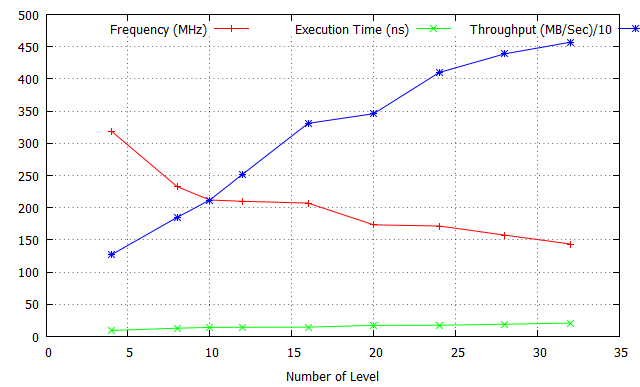
\includegraphics[width=8cm]{Figures/result1.png}
      \caption{Pipeline design overview}
    \label{result1}
\end{figure}

Figure \ref{result1} illustrates the graphical presentation of different efficiency parameter with variation of $\beta$. From the figure, it is clear that frequency and execution time smoothly either decrease or increase (respectively) with the increase of $\beta$. But, the throughput increases very sharply with the increase of $\beta$.



\section{Conclusion and Future Work}
We implement a web based anomaly detection device. The anomaly is detected based on score calculation. The incoming network packets are captured and parse the packets. The entire anomaly detection engine is based on software. Only the hardware part is the prioritization of anomalous packets.

We propose a hardware realization of parallel binary heap as an application of web based anomaly prioritization. The heap is implemented in pipelined fashion in FPGA platform. The propose design takes $O(1)$ time for all operations by ensuring minimum waiting time between two consecutive operations. We present the various design issues and hardware complexity. We explicitly analyze the design trade-offs of the proposed priority queue implementations.

The work presented in this paper leaves several directions for future research. We presented some of these idea here. (a) The interface we provide is essentially two parts: one is software part and the other is hardware one. The software part is responsible to parsing network packets and find some score based on some models. The hardware part provides an interface to make priority for the detected anomalous packets.It would be great idea if we can implement the detection part in hardware. In that case, we can achieve high throughput. (b) Due to limitation of on chip memory, we can not implement register based on chip memory for large number of nodes. We need to limit the number of nodes to be processed. Some authors have used off-chip memory which makes the system slow. We can improve this part.


\begin{thebibliography}{1}

\bibitem{pq0}S. Prasad, “Efficient parallel algorithms and data structures for discreteevent
simulation,” PhD Dissertation, 1990.

\bibitem{pq1} Sushil Prasad , I. Sagar Sawant 1995. Parallel Heap: A Practical Priority Queue for Fine-to-Medium-Grained Applications on Small Multiprocessors. Proceedings of 7th IEEE Symposium on Parallel and Distributed Processing (SPDP)1995.

\bibitem{pq2}	Xi He, Dinesh Agarwal, Sushil K. Prasad: "Design and implementation of a parallel priority queue on many-core architectures". HiPC 2012: 1-10

\bibitem{pq3} N. Deo and S. Prasad, “Parallel heap: An optimal parallel priority queue,” The Journal of Supercomputing, vol. 6, no. 1, pp. 87–98, 1992.

\bibitem{pq4} G. S. Brodal, J. L. Tradff, and C. D. Zaroliagis, “A parallel priority queue with constant time operations,” Journal of
Parallel and Distributed Computing, vol. 49, no. 1, pp. 4 – 21, 1998.

\bibitem{pq5} A. V. Gerbessiotis and C. J. Siniolakis, “Architecture independent parallel selection with applications to parallel
priority queues,” Theoretical Computer Science, vol. 301, no. 1 ¸ Vol 3, pp. 119 – 142, 2003.

\bibitem{pq6}	V. Nageshwara Rao, Vipin Kumar: "Concurrent Access of Priority Queues", IEEE Trans. Computers 37(12): 1657-1665 (1988)


\bibitem{hw1} S.-W. Moon, J. Rexford, and K. G. Shin, “Scalable hardware priority queue architectures for high-speed
packet switches,” IEEETC: IEEE Transactions on Computers, vol. 49, 2000.

\bibitem{hw2} R. Bhagwan and B. Lin, “Fast and scalable priority queue architecture for high-speed network switches,”
in INFOCOM, 2000, pp. 538–547.

\bibitem{hw3} H. J. Chao and N. Uzun, “A VLSI sequencer chip for ATM traffic shaper and queue manager,” IEEE
Journal of Solid-State Circuits, vol. 27, no. 11, pp. 1634–1642, November 1992.

\bibitem{hw5} K. Mclaughlin, S. Sezer, H. Blume, X. Yang, F. Kupzog, and T. G. Noll, “A scalable packet sorting circuit for high-speed
wfq packet scheduling,” IEEE Transactions on Very Large Scale Integration Systems, vol. 16, pp. 781–791, 2008.

\bibitem{hw6} H. Wang and B. Lin, “Succinct priority indexing structures for the management of large priority queues,” in Quality of
Service, 2009. IWQoS. 17th International Workshop on, july 2009, pp. 1 –5.

\bibitem{hw7} X. Zhuang and S. Pande, “A scalable priority queue architecture for high speed network processing,” in INFOCOM 2006. 25th IEEE International Conference on Computer Communications. Proceedings, april 2006, pp. 1 –12.

\bibitem{hw8} S.-W. Moon, K. Shin, and J. Rexford, “Scalable hardware priority queue architectures for high-speed packet switches,”
in Real-Time Technology and Applications Symposium, 1997. Proceedings., Third IEEE, jun 1997, pp. 203 –212.

\bibitem{hw9} R. Chandra and O. Sinnen, “Improving application performance with hardware data structures,” in Parallel Distributed Processing, Workshops and Phd Forum (IPDPSW), 2010 IEEE International Symposium on, april 2010, pp. 1 –4.
	
\bibitem{hw10} Yehuda Afek, Anat Bremler-Barr, Liron Schiff: Recursive design of hardware priority queues. Computer Networks 66: 52-67 (2014)

\bibitem{fpga1} A. Ioannou and M. G. Katevenis, “Pipelined heap (priority queue) management for advanced scheduling in high-speed networks,” IEEE/ACM Transactions on Networking (ToN), vol. 15, no. 2, pp. 450–461, 2007.

\bibitem{fpga2} Muhuan Huang, Kevin Lim, Jason Cong: A scalable, high-performance customized priority queue. FPL 2014: 1-4

\bibitem{fpga3} P. Kuacharoen, M. Shalan, and V. J. Mooney, “A configurable hardware scheduler for real-time sys-
tems,” in Engineering of Reconfigurable Systems and Algorithms, T. P. Plaks, Ed. CSREA Press, 2003,
pp. 95–101.




\bibitem{ah1} Abhishek Das, David Nguyen, Joseph Zambreno, Gokhan Memik, Alok N. Choudhary:
An FPGA-Based Network Intrusion Detection Architecture. IEEE Transactions on Information Forensics and Security 3(1): 118-132 (2008)

\bibitem{ah2} Abhishek Das, Sanchit Misra, Sumeet Joshi, Joseph Zambreno, Gokhan Memik, Alok N. Choudhary:
An Efficient FPGA Implementation of Principle Component Analysis based Network Intrusion Detection System. DATE 2008: 1160-1165

\bibitem{ah3} Sailesh Pati, Ramanathan Narayanan, Gokhan Memik, Alok N. Choudhary, Joseph Zambreno:
Design and Implementation of an FPGA Architecture for High-Speed Network Feature Extraction. FPT 2007: 49-56

\bibitem {Moh}	M. Abadeh, J. Habibi, Z. Barzegar, and M. Sergi, ``A parallel genetic local search algorithm for intrusion detection in computer networks," Eng. Appl. of AI, Vol. 20, No. 8, pp. 1058-1069, 2007.

\bibitem {web} Christopher Krügel, Giovanni Vigna: "Anomaly detection of web-based attacks". ACM Conference on Computer and Communications Security 2003: 251-261



\bibitem {35} J. Cannady, ``Artificial neural networks for misuse detection," in Proc. of
the National Information Systems Security Conference, Arlington, VA, 1998, pp. 443-456.

\bibitem {1} Varun Chandola, Arindam Banerjee, and Vipin Kumar, ``Anomaly detection: A survey," ACM Comput. Surv. Vol.41, No. 3, pp. 1-58, 2009.

\bibitem {Chr}	C. Krugel, G. Vigna, and W. Robertson, ``A multi-model approach to the detection of web-based attacks," Computer Networks, Vol. 48, No. 5, pp. 717-738, 2005.

\bibitem {Das} K. Das, and J. Schneider, ``Detecting anomalous records in categorical datasets," in Proc. of the 13th ACM SIGKDD International Conference on Knowledge Discovery and Data Mining, New
York, USA, 2007, pp. 220-229.

\bibitem {62} H. Debar, M. Becker, and D. Siboni, ``A neural network component for
an intrusion detection system," in IEEE Computer Society Symposium on Research
in Security and Privacy, Oakland, CA, USA, 1992, pp. 240-250.

\bibitem {68} D. Denning, ``An intrusion-detection model," IEEE Trans. on Software Engineering, Vol. 13, No. 2, pp. 222-232, 1987.


\bibitem {Fre} F. Valeur, D. Mutz, and G. Vigna, ``A Learning-Based Approach to the Detection of SQL Attacks, DIMVA, 2005, pp. 123-140.

\bibitem {111} J. Hochberg, K. Jackson, C. Stallings, and J. Mcclary, ``An automated system for detecting network intrusion and misuse," Computers \& Security, Vol.12, No. 3, pp. 235-248, 1993.

\bibitem {Janakiram} D. Janakiram, V. Reddy, and A. Kumar, ``Outlier detection in wireless sensor networks using Bayesian belief networks," in Proc. of the 1st International Conference on Communication System Software
and Middleware, 2006, pp. 1-6.

\bibitem {Meh} M. Kiani, A. Clark, and G. Mohay, ``Evaluation of Anomaly Based Character Distribution Models in the Detection of SQL Injection Attacks," ARES 2008, pp. 47-55.

\bibitem {160} S. Lee, and D. Heinbuch, ``Training a neural-network based intrusion detector
to recognize novel attacks," IEEE Transactions on Systems, Man \& Cybernetics, Vol. 31, No. 4, pp. 294-299, 2001.

\bibitem {198} S. Mukkamala, G. Janoski, and A. Sung, ``Intrusion detection using neural
networks and support vector machines," in 2002 International Joint Conference on
Neural Networks (IJCNN), Honolulu, HI, USA, 2002, pp. 1702-1707.

\bibitem {Kon} K. Rieck, and P. Laskov, ``Language models for detection of unknown attacks in network traffic," Journal in Computer Virology, Vol. 2, No. 4, pp. 243-256, 2007.

\bibitem {Wil}	W. Robertson, G. Vigna, C. Krugel, R. Kemmerer, ``Using Generalization and Characterization Techniques in the Anomaly-based Detection of Web Attacks, NDSS, 2006.

\bibitem {gio} G. Vigna, F. Valeur, D. Balzarotti, W. Robertson, C. Kruegel, and E. Kirda, ``Reducing errors in the anomaly-based detection of web-based attacks through the combined analysis of web requests and SQL queries,", Journal of Computer Security, Vol.17, No. 3, pp. 305-329, 2009.

\bibitem{baum} L. Rabiner, ``A tutorial on hidden Markov model and
selected applications in speech recognition", in Proc. of IEEE, Vol. 77, No. 2, pp. 257- 286, 1989.

\end{thebibliography}




% that's all folks
\end{document}


